\section{Optimisasi CMA-ES}

\begin{frame}{CMA-ES: Gambaran Umum}
    \textbf{Covariance Matrix Adaptation Evolution Strategy (CMA-ES)}
    \vspace{0.5cm}
    \begin{itemize}
        \item Algoritma optimisasi numerik stokastik tanpa turunan yang kuat.
        \item \textbf{Tipe:} Algoritma Evolusioner (domain kontinu).
        \item \textbf{Kasus Penggunaan:} Fungsi objektif non-konveks, tidak terkondisi dengan baik, multimodal, atau berisik.
        \item \textbf{Relevansi dengan VQE:} Digunakan untuk mengoptimalkan parameter $\boldsymbol{\theta}$ dari sirkuit variasional ketika gradien sulit dihitung atau berisik (misalnya, pada perangkat keras NISQ).
    \end{itemize}
\end{frame}

\begin{frame}{Cara Kerja CMA-ES}
    Algoritma mempertahankan distribusi Gaussian $\mathcal{N}(m, \sigma^2 C)$ dan memperbaruinya secara iteratif:
    \vspace{0.3cm}
    \begin{enumerate}
        \item \textbf{Pengambilan Sampel:} Menghasilkan populasi solusi kandidat baru (keturunan) dari distribusi saat ini.
        \item \textbf{Seleksi:} Mengevaluasi kebugaran (energi) dan memilih kandidat terbaik.
        \item \textbf{Adaptasi:} Memperbarui parameter distribusi:
            \begin{itemize}
                \item \textbf{Mean ($m$):} Bergerak menuju solusi yang lebih baik.
                \item \textbf{Ukuran Langkah ($\sigma$):} Mengontrol eksplorasi vs. eksploitasi.
                \item \textbf{Matriks Kovarian ($C$):} Mempelajari bentuk lanskap (korelasi antar variabel) untuk memandu pencarian.
            \end{itemize}
    \end{enumerate}
\end{frame}

\begin{frame}{Ilustrasi CMA-ES: Langkah 1}
    \begin{center}
        \textbf{Inisialisasi} \\
        Pencarian dimulai dengan mean awal dan distribusi yang luas.
        \vspace{0.5cm}
        
        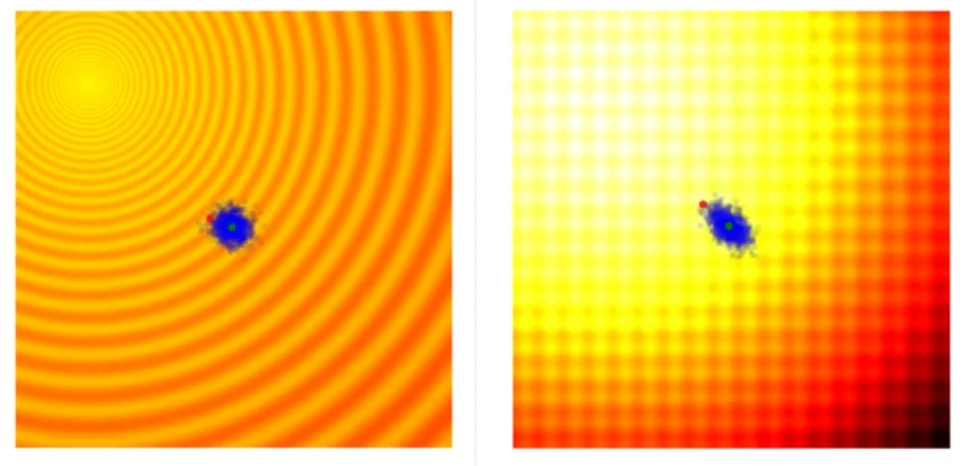
\includegraphics[width=0.7\textwidth]{Step1.png}
    \end{center}
\end{frame}

\begin{frame}{Ilustrasi CMA-ES: Langkah 2}
    \begin{center}
        \textbf{Pengambilan Sampel \& Seleksi} \\
        Kandidat diambil sampelnya; yang terbaik (biru) dipilih untuk memandu pembaruan.
        \vspace{0.5cm}
        
        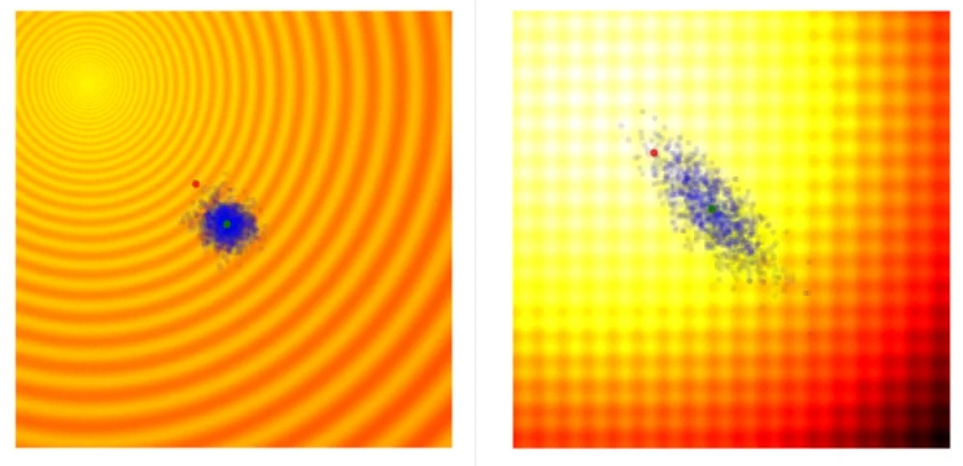
\includegraphics[width=0.7\textwidth]{Step2.png}
    \end{center}
\end{frame}

\begin{frame}{Ilustrasi CMA-ES: Langkah 3}
    \begin{center}
        \textbf{Adaptasi} \\
        Distribusi bergeser dan membentuk ulang (pembaruan kovarian) menuju lembah.
        \vspace{0.5cm}
        
        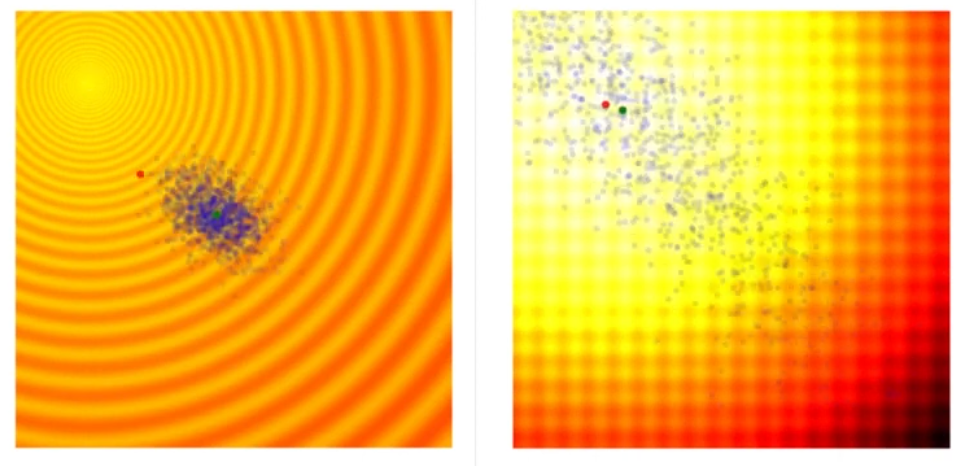
\includegraphics[width=0.7\textwidth]{Step3.png}
    \end{center}
\end{frame}

\begin{frame}{Ilustrasi CMA-ES: Langkah 4}
    \begin{center}
        \textbf{Eksplorasi} \\
        Algoritma mengeksplorasi lanskap, memanjang sepanjang arah optimal.
        \vspace{0.5cm}
        
        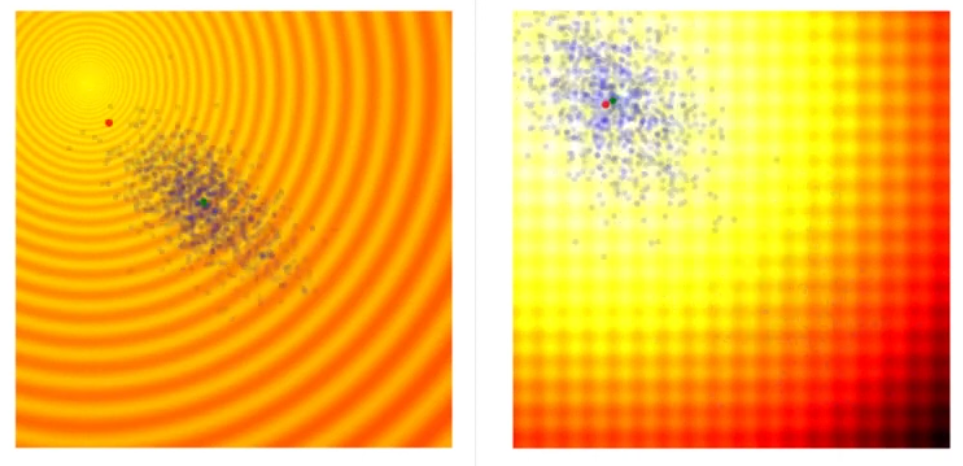
\includegraphics[width=0.7\textwidth]{Step4.png}
    \end{center}
\end{frame}

\begin{frame}{Ilustrasi CMA-ES: Langkah 5}
    \begin{center}
        \textbf{Konvergensi Dimulai} \\
        Ukuran langkah menurun saat populasi berpusat pada minimum.
        \vspace{0.5cm}
        
        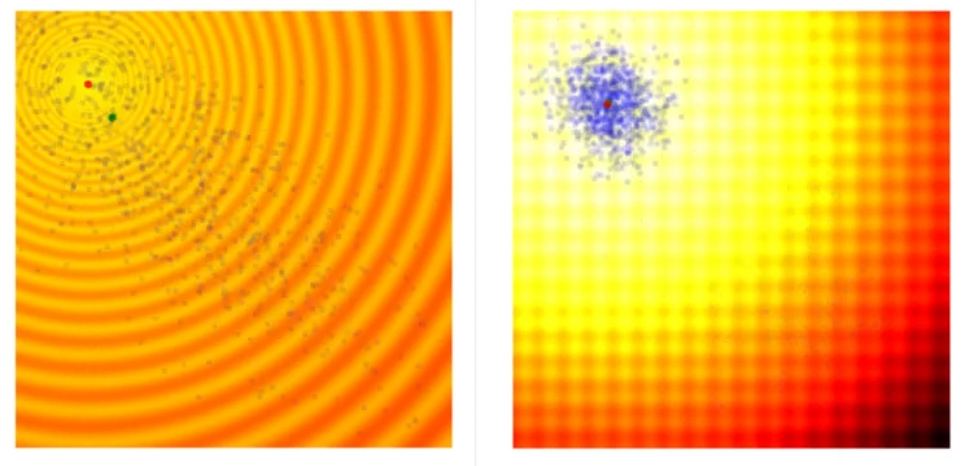
\includegraphics[width=0.7\textwidth]{Step5.png}
    \end{center}
\end{frame}

\begin{frame}{Ilustrasi CMA-ES: Langkah 6}
    \begin{center}
        \textbf{Penyetelan Halus} \\
        Lokalisasi presisi dari optimum.
        \vspace{0.5cm}
        
        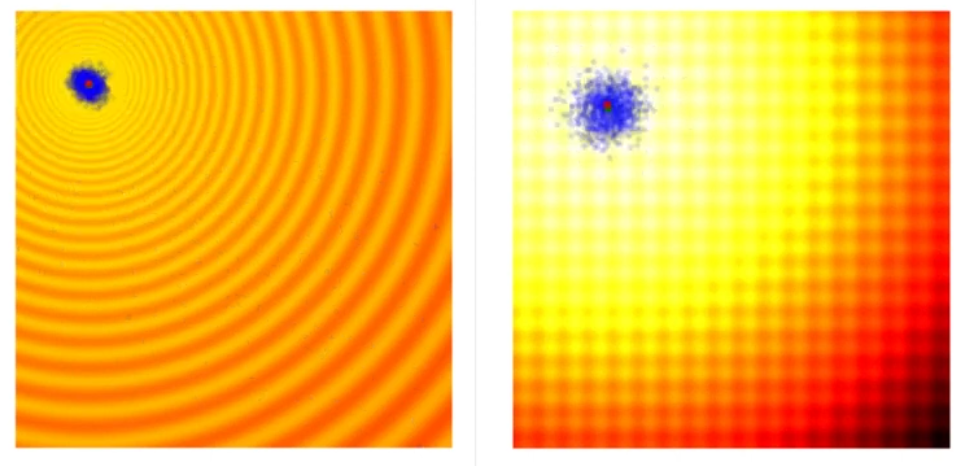
\includegraphics[width=0.7\textwidth]{Step6.png}
    \end{center}
\end{frame}

\begin{frame}{Ilustrasi CMA-ES: Langkah 7}
    \begin{center}
        \textbf{Optimisasi Selesai} \\
        Distribusi konvergen ke minimum global.
        \vspace{0.5cm}
        
        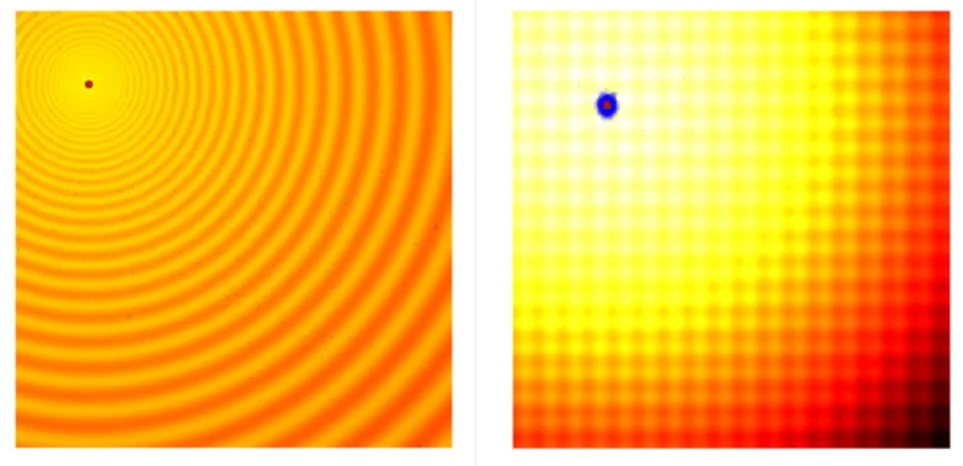
\includegraphics[width=0.7\textwidth]{Step7.png}
    \end{center}
\end{frame}
